\documentclass[russian,english]{llncs}
\usepackage[utf8]{inputenc}
\usepackage[T2A]{fontenc}
\usepackage[final]{graphicx}
\usepackage{epstopdf}
\usepackage[labelsep=period]{caption}
\usepackage[hyphens]{url}
\usepackage{amssymb,amsmath,mathrsfs}
\usepackage[russian,english]{babel}
%\usepackage{multicol}
\usepackage[ruled,vlined,linesnumbered,algo2e]{algorithm2e}
%\usepackage{algorithm}
%\usepackage[noend]{algorithmic}
\usepackage{color}
\usepackage{cmap}
\usepackage{array}

\tolerance=1000
\hbadness=5000
\newcommand{\const}{\mathrm{const}}
\newcommand{\tsum}{\mathop{\textstyle\sum}\limits}
\newcommand{\tprod}{\mathop{\textstyle\prod}\limits}
\newcommand{\cov}{\mathop{\rm cov}\limits}
\newcommand{\Dir}{\mathop{\rm Dir}\nolimits}
\newcommand{\norm}{\mathop{\rm norm}\limits}
\newcommand{\KL}{\mathop{\rm KL}\nolimits}
%\renewcommand{\geq}{\geqslant}
%\renewcommand{\leq}{\leqslant}
\newcommand{\eps}{\varepsilon}
\newcommand{\cond}{\mspace{3mu}{|}\mspace{3mu}}
\newcommand{\Loss}{\mathscr{L}}
\newcommand{\RR}{\mathbb{R}}
\newcommand{\cL}{\mathscr{L}}
\newcommand{\cP}{\mathscr{P}}
\newcommand{\kw}[1]{\textsf{#1}}
\SetKwFor{ForAll}{\textbf{for all}}{}{}

\begin{document}
%%Analysis of Images, Social Networks, and Texts
\title{
    Parallel Non-blocking Deterministic Algorithm for Online Topic Modeling
}
\author{
    Oleksandr Frei\inst{1}
    \and
    Murat Apishev\inst{2}
}
\institute{\noindent
    Moscow Institute of Physics and Technology,
    ~~\email{oleksandr.frei@gmail.com}
    \and
    National Research University Higher School of Economics,
    ~~\email{great-mel@yandex.ru}
}

\maketitle

\begin{abstract}
In this paper we present a new asynchronous algorithm for learning additively regularized topic models
and discuss the main architectural details of our implementation.
The key property of the new algorithm is that it behaves in a fully deterministic fashion,
which is typically hard to achieve in a non-blocking parallel implementation. The algorithm
had been
recently implemented in the BigARTM library (\texttt{http://bigartm.org}).
Our new algorithm is compatible with all features previously introduced in BigARTM library,
including multimodality, regularizers and scores calculation.
While the existing BigARTM implementation compares favorably
with the alternative packages such as Vowpal Wabbit or Gensim,
the new algorithm brings yet further improvements in CPU utilization,
memory usage, and spends even less time to achieve the same perplexity.

\vspace{1em}
\textbf{Keywords:}
    probabilistic topic modeling,
    Probabilistic Latent Sematic Analysis,
    Latent Dirichlet Allocation,
    Additive Regularization of Topic Models,
    stochastic matrix factorization,
    EM-algorithm,
    online learning,
    asynchronous and parallel computing,
    BigARTM.
\end{abstract}

\section{Introduction}
%
%\cite{li13parserver}

Topic models \cite{blei12ptm} is a powerful machine learning technology for statistical text analysis
that has been widely used in text mining, information retrieval, network analysis and other areas \cite{daud10knowledge}.
Today a lot of research efforts around topic models is devoted to distributed implementations of
\emph{Latent Dirichlet Allocation} (LDA)~\cite{blei03latent},
a specific Bayesian topic model that uses Dirichlet conjugate prior.
This lead to numerous implementations such as
AD-LDA~\cite{newman09distributed}, PLDA~\cite{wang09plda} and PLDA{+}~\cite{liu11plda},
all designed to run on a big cluster.
Largest topic models of web scale can reach millions of topics and vocabulary words, 
yielding Big Data models with trillions of parameters \cite{yuan15lightlda}.
Yet not all researchers and application are dealing with so large web-scale collections,
and they require an efficient implementation that can run on a powerful workstation or even laptop.
Such implementations are also very useful,
as shown by popular open-source packages
Vowpal Wabbit~\cite{langford07vw}, Gensim~\cite{rehurek10software} and Mallet~\cite{McCallum02mallet},
which are neither distributed nor sometimes even multi-threaded.

Scaling down a distributed algorithm can be challenging.
LightLDA~\cite{yuan15lightlda} is a major step in this direction,
however it is focused on the LDA model.
Our goal is to develop a flexible framework that can learn a wide variety of topic models.

BigARTM~\cite{vfardi15aist} is an open-source library for
regularized multimodal topic modeling of large collections.
BigARTM is based on a novel technique of additive regularized topic models (ARTM) \cite{voron14dan-eng,voron14mlj,voron14aist},
which gives flexible multi-criteria approach to probabilistic topic modeling.
ARTM includes all popular models such as 
LDA~\cite{blei03latent}, 
PLSA~\cite{hofmann99plsi},
and many others.
Key feature of ARTM is that it provides a cohesive framework that allows users to combine
different topic models that previously did not fit together.

BigARTM is proven to be very fast comparing to the alternative packages.
According to~\cite{vfardi15aist}, BigARTM
runs approx. $10$ times faster comparing to Gensim~\cite{rehurek10software}
and twice faster than
Vowpal Wabbit (VW)~\cite{langford07vw}
in a single thread.
With multiple threads BigARTM wins even more
as it scales linearly at least up to 16 threads.
In this paper we address the remaining limitations of the library,
including few performance bottlenecks
and fixing non-deterministic behavior of the Online algorithm.

%Deterministic behavior is an important property for any algorithm,
%including those of a stochastic nature.
%For the end users of a software system run-to-run reproducibility is a must-have property,
%because this is what they expect based on their previous experience.
%Indeed, refreshing a web-pages or re-doing an operation tend to
%produce an identical result, regardless of how much software complexity is hidden behind the scenes.
%For the researches determinism is also important
%because it enables them to reproduce their old experiments
%and study impact of various parameters on the result.
%Finally, for the developers of the algorithm
%determinism allow to reproduce bugs and write simple unit-tests with well-defined results.

%Determinism is particularly hard to achieve
%in concurrent implementations, because in a multi-threaded environment
%it might not be sufficient to just fix a random seed or an initial approximation.
%In this paper we present a deterministic modification of parallel non-blocking algorithm
%for online topic modeling, previously developed for BigARTM library.
%We implement new algorithm in BigARTM and demonstrate that new version converges faster
%than previous algorithm in terms of perplexity,
%yet being more efficient in CPU and memory usage.

The rest of the paper is organized as follows.
In~section~\ref{sec:Notation}
we introduce basic notation used throughout this paper.
In~sections~\ref{sec:Offline}, \ref{sec:Online}, \ref{sec:AsyncOnline}
we summarize Offline, Online and Asynchronous Online algorithms for learning ARTM models.
In~section~\ref{sec:Architecture}
we~compare the internal architecture of BigARTM library between versions v0.6 and v0.7.
In~section~\ref{sec:Experiments}
we~report results of our experiments on large datasets.
In~section~\ref{sec:Conclusions}
we~discuss advantages, limitations and open problems of BigARTM.

%sashafrey:
%really technical topics in my opinion does not belong to AISTconf article;
%it would be more appropriate to discuss the following in the full 12-page article in http://www.ispras.ru/en/ journal
%\begin{itemize}
%    \item Details of CLI interface and python interface, usage examples
%    \item List new features: coherence score and regularizer, classification, documents markdown (aka $p_{tdw}$ matrices)
%    \item Our technologies (Protobuf for low-level C API, Boost Serialize for import/export, GLog, GFlags, GTest, etc)
%    \item Our build solution and CI solution (CMake, Visual Studio, GitHub, Git submodules, Travis, Apveyour, Read-The-Docs)
%    \item Why people care about run-to-run reproducibility
%    https://software.intel.com/en-us/articles/consistency-of-floating-point-results-using-the-intel-compiler
%\end{itemize}

\section{Notation}
\label{sec:Notation}

Let
$D$ denote a finite set (collection) of texts and
$W$ denote a~finite set (vocabulary) of all terms from these texts.
Let
$n_{dw}$ denote the number of occurrences of a term $w \in W$ in a document $d \in D$;
$n_{dw}$ values form a sparse matrix of size $|W| \times |D|$,
known as \emph{bag-of-words} representation of the collection.

Given an $(n_{dw})$ matrix, a probabilistic topic model finds two matrices:
$\Phi~=~\{\phi_{wt}\}$ and $\Theta = \{\theta_{td}\}$,
of sizes $|W| \times |T|$ and $|T| \times |D|$ respectively,
where $|T|$ is a used-defined number of \emph{topics} in the model.
Matrices $\Phi$ and $\Theta$
provide a compressed representation of the $(n_{dw})$ matrix:
\[
n_{dw} \approx n_d \sum_{t \in T} \phi_{wt} \theta_{td}, \text { for all } d \in D, w \in W,
\]
where $n_d = \sum_{w \in W} n_{dw}$ denotes the total number of terms in a document $d$.

To learn $\Phi$ and $\Theta$ from $(n_{dw})$ an additively-regularized topic model (ARTM) maximizes
the log-likelihood, regularized via an additional penalty term $R(\Phi, \Theta)$:
\begin{gather}
\label{eq:ARTM}
    \sum_{d\in D}\sum_{w\in W} n_{dw} \ln \sum_{t\in T} \phi_{wt} \theta_{td} + R(\Phi, \Theta)
    \;\to\; \max_{\Phi,\Theta}.
\end{gather}
Regularization penalty $R(\Phi, \Theta)$ may incorporate external knowledge
of the expert about the collection.
With no regularization (${R=0}$) it corresponds to PLSA~\cite{hofmann99plsi}.
Many Bayesian topic models, including LDA~\cite{blei03latent}, can be represented
as special cases of ARTM with different regularizers~$R$,
as shown in~\cite{voron14mlj,voron14aist}.

In \cite{voron14dan-eng} it is shown that the \mbox{local} maximum $(\Phi,\Theta)$
of the problem~\eqref{eq:ARTM} satisfies
the following system of equations:
\begin{align}
    \label{eq:Estep}
    p_{tdw} &= \norm_{t\in T} \bigl(\phi_{wt}\theta_{td}\bigr);
\\
    \label{eq:Mstep:phi}
    \phi_{wt} &= \norm_{w\in W}
        \biggl(
            n_{wt} + \phi_{wt} \frac{\partial R}{\partial \phi_{wt}}
        \biggr);
        \quad
            n_{wt} = \sum_{d\in D} n_{dw} p_{tdw};
%    \phi_{wt} &= \norm_{w\in W}
%        \biggl(
%            n_{wt} + r_{wt}
%        \biggr);
%    \quad
%    n_{wt} = \sum_{d\in D} n_{dw} p_{tdw};
%    \quad
%    r_{wt} = \phi_{wt} \frac{\partial R}{\partial \phi_{wt}};
\\
    \label{eq:Mstep:theta}
    \theta_{td} &= \norm_{t\in T}
        \biggl(
            n_{td} + \theta_{td} \frac{\partial R}{\partial \theta_{td}}
        \biggr);
        \quad\quad
            n_{td} = \sum_{w\in d} n_{dw} p_{tdw};
%    \theta_{td} &= \norm_{t\in T}
%        \biggl(
%            n_{td} + r_{td}
%        \biggr);
%    \quad
%    r_{td} = \theta_{td} \frac{\partial R}{\partial \theta_{td}};
        %\sum_{m=1}^M \tau_m \!\!\sum_{w\in W^m}\!\!\! n_{dw} p_{tdw};
\end{align}
where operator
$\norm_{i \in I} x_i = \frac{\max\{x_i,0\}}{\sum\limits_{j\in I} \max\{x_j,0\}}$
transforms a~vector $(x_i)_{i \in I}$ to a~discrete distribution,
$n_{wt}$ counters represent term frequency of word $w$ in topic $t$.
% Hard to make up a similar explanation for $n_{td}$. Thesse counters represent "document frequency"? No...

Learning of $\Phi$ and $\Theta$ from \eqref{eq:Estep}--\eqref{eq:Mstep:theta} can be done by EM-algorithm,
which starts from a random values in $\Phi$ and $\Theta$, and iterates
E-step \eqref{eq:Estep} and
M-steps \eqref{eq:Mstep:phi},\eqref{eq:Mstep:theta}
until convergence.
% Simple-iteration method - skip for now
In the sequel we discuss several variations of such EM-algorithm,
which are all based on the above formulas but differ in the way how operations are ordered and grouped together.

%In additional to plain text many collections has additional data,
%such as authors, class or category labels, date-time stamps.
%In \cite{vfardy15cikmtm} this data can be represented as \emph{modalities},
%where the overall vocabulary $W$ is split into $M$ subsets
%$W = W^1 \sqcup \dots \sqcup W^M$, one subset per modality,
%and $\Phi$ matrix is normalized independently within each modality:
%\begin{align}
%    \sum_{w \in W^m} \phi_{wt} = 1, \; \text{ for all } t \in T, m = 1, \dots, M \\\notag
%\end{align}


\section{Offline algorithm}
\label{sec:Offline}

\SetAlgoSkip{}
\begin{algorithm2e}[t]
\caption{Offline algorithm}
\label{alg:Offline}
\BlankLine
\KwIn{collection $D$;}
\KwOut{matrix $\Phi = (\phi_{wt})$;}
\BlankLine
initialize $(\phi_{wt})$\;
create batches $D := D_1 \sqcup D_2 \sqcup \dots \sqcup D_B$\;
\label{alg:Offline:FormBatches}
\Repeat{$(\phi_{wt})$ converges}{
    %$\tilde n_{wt} := 0$ for all $w \in W$ and $t \in T$\;
    %\ForAll{documents $d \in D$} {
    %    $(\tilde n_{wt}) := (\tilde n_{wt}) + \kw{ProcessDocument}(d, \Phi)$\;
    %}
    $(n_{wt}) := \mathlarger\sum\limits_{b=1, \dots, B} \; \mathlarger\sum\limits_{d \in D_b} \; \kw{ProcessDocument}(d, \Phi)$\;
    \label{alg:Offline:Normalize}
    $(\phi_{wt}) := \norm_{w \in W} (n_{wt} + \phi_{wt} \frac{\partial R}{\partial \phi_{wt}})$\;
}
\end{algorithm2e}
\begin{algorithm2e}[t]
\caption{\kw{ProcessDocument}($d, \Phi$)}
\label{alg:ProcessDocument}
\BlankLine
\KwIn{document $d \in D$, matrix $\Phi=(\phi_{wt})$;}
\KwOut{matrix $(\tilde n_{wt})$, vector $\theta_{td}$;}
\BlankLine
initialize $\theta_{td} := \frac{1}{|T|}$ for all $t \in T$\;
\Repeat{$\theta_d$ converges}{
    \label{alg:ProcessDocument:innerLoopBegin}
    $p_{tdw} := \norm_{t\in T} \bigl(\phi_{wt}\theta_{td}\bigr)$ for all $w\in d$ and $t \in T$\;
    $\theta_{td} := \norm_{t\in T}
        \bigl(
            \sum_{w\in d} n_{dw} p_{tdw} + \theta_{td} \frac{\partial R}{\partial \theta_{td}}
        \bigr)$ for all $t \in T$\;
}
\label{alg:ProcessDocument:innerLoopEnd}
$\tilde n_{wt} := n_{dw} p_{tdw}$ for all $w \in d$ and $t \in T$\;
\end{algorithm2e}

\begin{figure}[t]
\centering
\begin{tabular}{c}
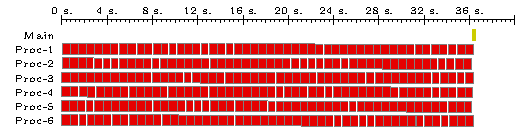
\includegraphics[height=4cm, width=12cm]{plots/offline.pdf} \\
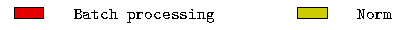
\includegraphics[scale=1]{plots/legend_offline.pdf}
\end{tabular}
\caption{Gantt chart for execution of the Offline algorithm} \label{fig:gantt:offline}
\end{figure}

The algorithm is given by
Fig. \ref{alg:Offline} (\kw{Offline algorithm}) and
Fig. \ref{alg:ProcessDocument} (\kw{ProcessDocument}).

Subroutine \kw{ProcessDocument($d, \Phi$)} corresponds to equations \eqref{eq:Estep} and \eqref{eq:Mstep:theta} from the solution of the ARTM optimization problem \eqref{eq:ARTM}.
\kw{ProcessDocument} requires a fixed $\Phi$ matrix
and a vector $n_{dw}$ of term frequencies for a given document $d \in D$,
and as a result it returns the topical distribution $\theta_{td}$ for the document,
and a matrix $(\hat n_{wt})$ of size $|d| \times |T|$,
where $|d|$ gives the number of distinct terms in the document.
The \kw{ProcessDocument} might be also useful as a separate routine which finds $\theta_{td}$ distribution for a new document,
but in the \kw{Offline algorithm} it is rather used as a building block in an iterative EM-algorithm that learns the $\Phi$ matrix.

The \kw{Offline algorithm} performs multiple scans over the collection, calls \kw{ProcessDocument}
for each document $d \in D$ from the collection,
and then aggregates the resulting $(\hat n_{wt})$ matrices into the final $(n_{wt})$ matrix of size $|W| \times |T|$.
After each scan it recalculates $\Phi$ matrix according to the equation $\eqref{eq:Mstep:phi}$.

%To split collection into batches and process them concurrently is a common approach,
%introduced in AD-LDA algorithm \cite{newman09distributed}, and
%then further developed in PLDA \cite{wang09plda} and PLDA{+} \cite{liu11plda} algorithms.

At step \ref{alg:Offline:FormBatches} we split collection $D$ into batches $(D_b)$.
This step is not strictly necessary for the \kw{Offline algorithm},
and it rather reflects an internal implementation detail.
For performance reasons the outer loop over batches $b = 1, \dots, B$ is parallelized across multiple threads,
and within each batch the inner loop $d \in D_b$ is executed in a single thread.
Each batch is stored in a separate disk file on disk to allow out-of-core streaming of the collection.
For typical collections it is reasonable to have around $1000$ documents per batch,
however for ultimate performance we encourage users to experiment with this parameter.
Too small batches can cause disk IO overhead due to lots of small reads,
while too large batches will result in bigger tasks that will not be distributed evenly across computation threads.

Note that $\theta_{td}$ values appear only within $\kw{ProcessDocument}$ subroutine.
This leads to efficient memory usage because the implementation never stores the entire theta matrix at any given time.
Instead, $\theta_{td}$ values are recalculated from scratch on every pass through the collection.

Fig. \ref{fig:gantt:offline} illustrates a run-time behavior of the \kw{Offline algorithm}.
It shows a Gantt chart, where boxes correspond to the time spent in processing an individual batch.
The final box, executed on the main thread, correspond to the time spent in the step \ref{alg:Offline:Normalize}
to normalize $n_{wt}$ values and produce a new $\Phi$ matrix.

\section{Online algorithm}
\label{sec:Online}

\SetAlgoSkip{}
\begin{algorithm2e}[t]
	\caption{Online algorithm} %\mbox{regularized} topic modeling
	\label{alg:Online}
	\BlankLine
	\KwIn{collection $D$, parameters $\eta, \tau_0, \kappa$;}
	\KwOut{matrix $\Phi = (\phi_{wt})$;}
	\BlankLine
	create batches $D := D_1 \sqcup D_2 \sqcup \dots \sqcup D_B$\;
	initialize $(\phi^0_{wt})$\;
	\ForAll{update $i = 1, \dots, \lfloor B / \eta \rfloor$} {
		$(\hat n^i_{wt}) := \kw{ProcessBatches}(\{D_{\eta (i - 1) + 1}, \dots, D_{\eta i}\}, \Phi^{i - 1})$\;
		$\rho_i := (\tau_0 + i)^{-\kappa}$\;
		\label{alg:Online:Rho}
		$(n^{i}_{wt}) := (1 - \rho_i) \cdot (n^{i-1}_{wt}) + \rho_i \cdot (\hat n^{i}_{wt})$\;
		\label{alg:Online:Merge}
		$(\phi^{i}_{wt}) := \norm_{w \in W} (n^{i}_{wt} + \phi^{i - 1}_{wt} \frac{\partial R}{\partial \phi_{wt}})$\;
		\label{alg:Online:Normalize}
	}
\end{algorithm2e}
\begin{figure}[t!]
	\centering
	\begin{tabular}{c}
		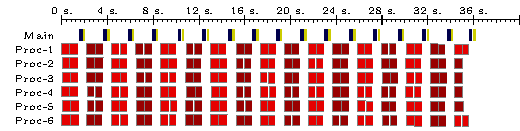
\includegraphics[height=4cm, width=12cm]{plots/online.pdf} \\
		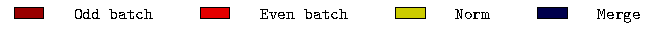
\includegraphics[scale=1]{plots/legend_online.pdf}
	\end{tabular}
	\caption{Gantt chart for new online algorithm} \label{fig:gantt:online}
\end{figure}

The \kw{Online algorithm} (Fig. \ref{alg:Online}), originally suggested in \cite{hoffman10online},
improves the convergence rate of the \kw{Offline algorithm}
by re-calculating matrix $\Phi$ after every $\eta$ batches.
To simplify the notation
we introduce a trivial subroutine
\[
\kw{ProcessBatches}(\{D_b\}, \Phi) = \mathlarger\sum\limits_{D_b} \mathlarger\sum\limits_{d \in D_b} \; \kw{ProcessDocument}(d, \Phi) \\
\]
that aggregates the output of $\kw{ProcessDocument}$ across specific set of batches at a constant $\Phi$ matrix.
The algorithm is then given by Fig. \ref{alg:Online}.
Here the split of the collection $D := D_1 \sqcup D_2 \sqcup \dots \sqcup D_B$
into batches
plays far more significant role than in the \kw{Offline algorithm},
because different splitting algorithmically affects the result.
At step \ref{alg:Online:Merge} the new $n_{wt}^{i+1}$ values are calculated as a convex combination
of the old values $n_{wt}^{i}$ and the value $\hat n_{wt}^{i}$ produced on the recent batches.
Old counters $n_{wt}^{i}$ are discounted by a factor $(1 - \rho_i)$,
which depends on the iteration number. A common strategy is to use $\rho_i = (\tau_0 + i)^{-\kappa}$,
where typical values for $\tau_0$ are between $64$ and $1024$, for $\kappa$ --- between $0.5$ and $0.7$.

As in the \kw{Offline algorithm}, the outer loop over batches
$D_{\eta (i - 1) + 1}, \dots, D_{\eta i}$ is executed concurrently across multiple threads.
The problem with this approach is that all threads have no useful work to do during steps
\ref{alg:Online:Rho}-\ref{alg:Online:Normalize} of the \kw{Online algorithm}.
The threads can not start processing the next batches because a new version of $\Phi$ matrix is not ready yet.
As a result the CPU utilization stays low, and the run-time Gantt chart of the \kw{Online algorithm} typically looks like in Fig. \ref{alg:Online}.
The color indicate which version of the $p^i_{wt}$ matrix was used to process each batch
(orange for even $i$, yellow for odd $i$).
Blue box correspond to the time spend in merging $n_{wt}$ with $\hat n_{wt}$,
Green box is, as before, the time spent to normalize $n_{wt}$ values and produce a new $p_{wt}$ matrix.

In the next section we present an asynchronous non-blocking modification of the online algorithm that results in better CPU utilization.

\section{Asynchronous online algorithm}
\label{sec:AsyncOnline}

\SetAlgoSkip{}
\begin{algorithm2e}[t]
	\caption{Asynchronous online algorithm} %\mbox{regularized} topic modeling
	\label{alg:AsyncOnline}
	\BlankLine
	\KwIn{collection $D$, parameters $\eta, \tau_0, \kappa$;}
	\KwOut{matrix $\Phi = (\phi_{wt})$;}
	\BlankLine
	create batches $D := D_1 \sqcup D_2 \sqcup \dots \sqcup D_B$\;
	initialize $(\phi^0_{wt})$\;
	$F^1 := \kw{AsyncProcessBatches}(\{D_{1}, \dots, D_{\eta}\}, \Phi^0)$\;
	\label{alg:AsyncOnline:FirstStep}
	\ForAll{update $i = 1, \dots, \lfloor B / \eta \rfloor$} {
		\If{$i \neq \lfloor B / \eta \rfloor$}{
			\label{alg:AsyncOnline:IfStatement}
			$F^{i+1} := \kw{AsyncProcessBatches}(\{D_{\eta i + 1}, \dots, D_{\eta i + \eta}\}, \Phi^{i-1})$\;
		}
		$\hat n^i_{wt} := \kw{Await}(F^i)$\;
		$\rho_i := (\tau_0 + i)^{-\kappa}$\;
		$(n^{i}_{wt}) := (1 - \rho_i) \cdot (n^{i-1}_{wt}) + \rho_i \cdot (\hat n^{i}_{wt})$\;
		$(\phi^{i}_{wt}) := \norm_{w \in W} (n^{i}_{wt} + \phi^{i-1}_{wt} \frac{\partial R}{\partial \phi_{wt}})$\;
	}
\end{algorithm2e}

\begin{figure}[t]
	\centering
	\begin{tabular}{c}
		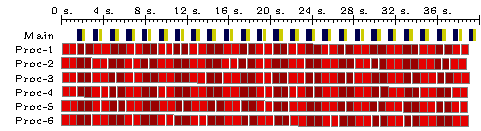
\includegraphics[height=4cm, width=12cm]{plots/async.pdf} \\
		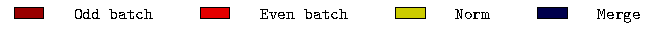
\includegraphics[scale=1]{plots/legend_online.pdf}
	\end{tabular}
	\caption{Gantt chart for async online algorithm} \label{fig:gantt:AsyncOnline}
\end{figure}

Asynchronous online algorithm is based on two new routines, \kw{AsyncProcessBatches} and \kw{Await}.
The first one is equivalent to \kw{ProcessBatches}, except that it just queues the task for an asynchronous execution and returns immediately.
Its output is a future object (for example, an \kw{std::future} from \kw{C++11} standard),
which can be later passed to $\kw{Await}$ in order to get the actual result, e.g. in our case the $\hat n_{wt}$ values.
In between calls to \kw{AsyncProcessBatches} and \kw{Await} the algorithm
can perform some other useful work, while the background threads are calculating the $\hat n_{wt}$ values.

The resulting algorithm is given by Fig. \ref{alg:AsyncOnline}.
To calculate $\hat n^{i+1}_{wt}$ it uses $\Phi^{i-1}$ matrix,
which is one generation older than $\Phi^{i}$ matrix used by the conventional \kw{Online algorithm} \ref{alg:Online}.
This adds an extra ``offset'' between the moment when $\Phi$ matrix is calculated and the moment when it is used,
and as a result gives the algorithm additional flexibility to distribute more payload to computation threads.
Steps \ref{alg:AsyncOnline:FirstStep} and \ref{alg:AsyncOnline:IfStatement} of the algorithm
are just technical tricks to implement the ``offset'' idea.

Adding an offset should negatively impact the convergence of the asynchronous algorithm \ref{alg:AsyncOnline}
comparing to the conventional algorithm \ref{Alg:Online}.
For example, in \kw{AsyncProcessBatches} the initial matrix $\Phi^0$ is used twice,
and the two last matrices $\Phi^{\lfloor B / \eta \rfloor - 1}$ and $\Phi^{\lfloor B / \eta \rfloor}$ will not be used at all.
%(except for $\Phi^{\lfloor B / \eta \rfloor}$ which forms the final result of the algorithm).
One the other hand the asynchronous algorithm gives better CPU utilization,
as clearly shown by the Gantt chart from Fig. \ref{fig:gantt:AsyncOnline}.
%The color scheme for the boxes is as in Fig. \ref{fig:gantt:AsyncOnline}.

This tradeoff convergence and CPU utilization is evaluated in the experiments from section \ref{sec:Experiments}.

\section{Implementation}
\label{sec:Architecture}

\begin{figure}[t]
	\begin{centering}
		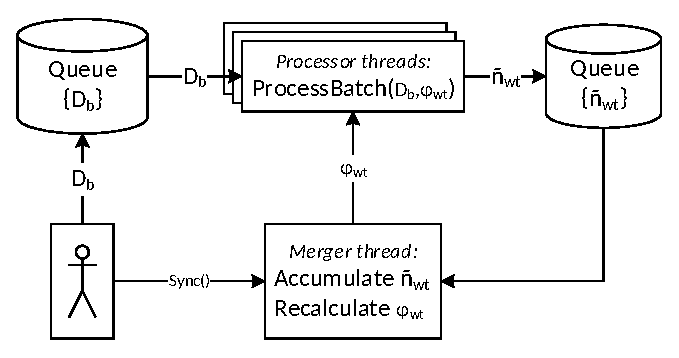
\includegraphics[height=39mm]{diagramm_artm_core.eps}
		\caption{Diagram of BigARTM components (old architecture)}
		\label{fig:diagramm_artm_core}
	\end{centering}
\end{figure}
\begin{figure}[t]
	\begin{centering}
		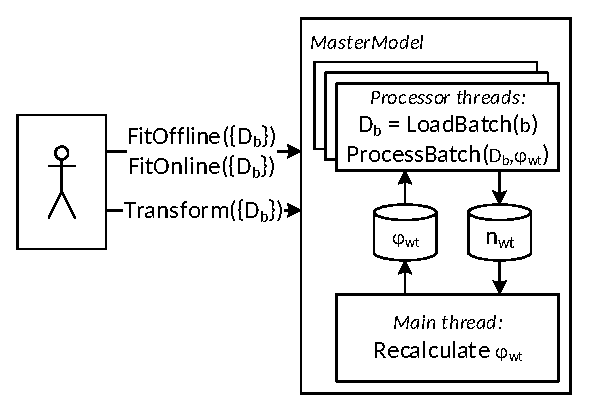
\includegraphics[height=54mm]{diagramm_artm_core_v07.eps}
		\caption{Diagram of BigARTM components (new architecture)}
		\label{fig:diagramm_artm_core_v07}
	\end{centering}
\end{figure}

The challenging part for the implementation is to aggregate the $\hat n_{wt}$ matrices across multiple batches, given that they are processed in different threads.
The way BigARTM solves this challenge was changed between versions \kw{v0.6} (see Fig. \ref{fig:diagramm_artm_core}) and \kw{v0.7} (see Fig. \ref{fig:diagramm_artm_core_v07}).
In the old architecture the $\hat n_{wt}$ matrices were stored in a queue, and then aggregated by a dedicated \emph{Merger thread}.
This often caused performance bottlenecks, particularly because of small batches or due to a small number of iterations in \kw{ProcessDocument}'s inner loop 
\ref{alg:ProcessDocument:innerLoopBegin}-\ref{alg:ProcessDocument:innerLoopEnd}.

In the new architecture we removed Merger thread, and $\hat n_{wt}$ are written directly into the final $n_{wt}$ matrix
concurrently from all processor threads.
To synchronize the write access we require that
no threads simultaneously update the same row in $\hat n_{wt}$ matrix,
yet the data for distinct words can be written in parallel.
This is enforced by spin locks $l_w$, one per each word in the dictionary $W$.
At the end of \kw{ProcessDocument} we loop through all $w \in d$, acquire the corresponding lock $l_w$, append $\hat n_{wt}$ to $n_{wt}$ and release the lock.
This approach is similar to \cite{smola10architecture},
where the same pattern is used to update a shared stated in a distributed topic modeling architecture.

In our new architecture we also removed \emph{DataLoader} thread, which previously was loading batches from disk.
Now this happens directly from processor thread, which simplified the architecture without sacrificing performance.

In addition, we provided a cleaner API so now the users may use simple \kw{FitOffline}, \kw{FitOnline} methods to learn the model,
and $\kw{Transform}$ to apply the model to the data.
Previously the users had to interact with low-level building blocks, such as \kw{ProcessBatches} routine.

\section{Experiments}
\label{sec:Experiments}

In this section we compare the effectiveness of the
\kw{Offline algorithm} (Fig. \ref{alg:Offline}),
\kw{Online algorithm} (Fig. \ref{alg:Online}),
asynchronous online algorithm (Fig. \ref{alg:AsyncOnline}),
and the old non-deterministic online algorithm from \kw{BigARTM v0.6}, described in \cite{vfardi15aist}.
According to \cite{vfardi15aist}, the later algorithm
runs ca. $10$ times comparing to Gensim~\cite{rehurek10software},
and twice faster comparing to 
Vowpal Wabbit (VW)~\cite{langford07vw}
in a single thread;
an with multiple threads BigARTM wins even more.

In the experiments we use \emph{Wikipedia} dataset ($|D| = 3.7m$ articles, $|W| = 100k$ words)
and \emph{Pubmed} dataset ($|D| = 8.2m$ abstracts, $|W| = 141k$ words).
The experiments ran on Intel Xeon CPU E5-2650 v2 system with 2 processors, 16 physical cores in total (32 with hyper-threading).


Fig. \ref{fig:perf} show the \emph{perplexity} as a function of the time spend by the four algorithms listed above.
%\kw{Offline algorithm} (Fig. \ref{alg:Offline}),
%\kw{Online algorithm} (Fig. \ref{alg:Online}),
%asynchronous online algorithm (Fig. \ref{alg:AsyncOnline}),
%and the old non-deterministic online algorithm from \kw{BigARTM v0.6}, described in \cite{vfardi15aist}.
The perplexity measure is defined as
\begin{equation}
\label{eq:perplexity}
\mathscr{P}(D, p) =
%\exp\left(- \frac{1}{n} L(\Phi, \Theta) \right) =
\exp \biggl( - \frac{1}{n} \sum_{d \in D} \sum_{w \in d} n_{dw} \ln \sum_{t\in T} \phi_{wt} \theta_{td} \biggr),
\end{equation}
 where $n = \sum_d n_d$. Lower perplexity means better result.
Each point on the figures corresponds to a moment when the algorithm finishes a complete scan of the collection.
Each algorithm was time-boxed to run for a 40 minutes for Wikipedia and 30 minutes for Pubmed.

\begin{figure}[t]
	\centering
	\begin{minipage}[b]{0.4\textwidth}
		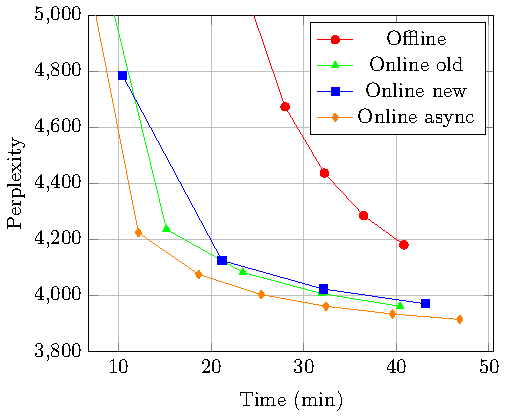
\includegraphics[scale=0.65]{plots/perplexity_time_plot_12.pdf}
	\end{minipage}
	$\qquad\quad$
	\begin{minipage}[b]{0.4\textwidth}
		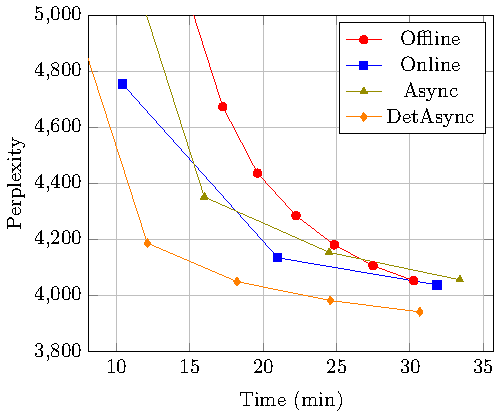
\includegraphics[scale=0.65]{plots/perplexity_time_plot_16.pdf}
%		\caption{12 physical cores, 40 minutes limit} \label{fig:compare12}
	\end{minipage}
	\caption{Perplexity versus time for Wikipedia (left) and Pubmed (right), $|T| = 100$ topics}
	\label{fig:perf}
\end{figure}

Table \ref{tab:memory} gives peak memory usage for $|T| = 1000$ topics model on Wikipedia and Pubmed datasets.
TDB: explain memory usage (how many matrices, what is the size of each matrix, how big batches affect memory usage, why old algorithm is so inefficient)

\begin{table}[h]
	\caption{
		BigARTM peak memory usage in GB, $|T| = 1000$ topics
	}
	\label{tab:memory}
	\centering\tabcolsep=4.3pt
	\begin{tabular}[t]{|l|cccc|}
		\hline
		& Offline   & Online    & Async     & Old online  \\
		\hline
		Pubmed	& {5.17}   	& {4.68}   	& {8.18}   	& {13.4}      \\
		Wiki	& {1.74}   	& {2.44}   	& {3.93}   	& {7.9}       \\ 
		\hline
	\end{tabular}
\end{table}



\section{Conclusions}
\label{sec:Conclusions}

%Our implementation is designed to be a building block in a distributed topic model,

TBD

\bigskip
\subsubsection*{Acknowledgements.}
\nopagebreak
The work was supported by Russian Science Foundation (grant 15-18-00091).

%%%%%%%%%%%%%%%%%%%%%%%%%%%%%%%%%%%%%%%%%%%%%%%%%%%%%%%%%%%%%%%%%%%%%%%%%%%%
%\bibliographystyle{splncs03}
%\bibliography{MachLearn}

\begin{thebibliography}{10}
%\providecommand{\url}[1]{\texttt{#1}}
%\providecommand{\urlprefix}{URL }

\bibitem{blei12ptm}
D.~M. Blei.
\newblock Probabilistic topic models.
\newblock {\em Communications of the ACM}, 55(4):77--84, 2012.

\bibitem{daud10knowledge}
Daud, A., Li, J., Zhou, L., Muhammad, F.: Knowledge discovery through directed
probabilistic topic models: a survey. Frontiers of Computer Science in China
4(2),  280--301 (2010)

%\bibitem{li13parserver}
%M.~Li, D.~G. Andersen, J.~W. Park, A.~J. Smola, A.~Ahmed, V.~Josifovski, J.~Long, E.~J. Shekita, and B.~Y. Su.
%\newblock{Scaling distributed machine learning with the parameter server.}
%\newblock{In Proc. OSDI}, pp. 583-598, 2013.

\bibitem{yuan15lightlda}
J.~Yuan, F.~Gao, Q.~Ho, W.~Dai, J.~Wei, X.~Zheng, E.~P. Xing, T.Y.~Liu, and W.~Y. Ma.
\newblock{LightLDA: Big Topic Models on Modest Computer Clusters.}
\newblock{In Proceedings of the 24th International Conference on World Wide Web}, pp. 1351-1361, 2015.

\bibitem{blei03latent}
D.~M. Blei, A.~Y. Ng, and M.~I. Jordan.
\newblock Latent {Dirichlet} allocation.
\newblock {\em Journal of Machine Learning Research}, 3:993--1022, 2003.

\bibitem{hofmann99plsi}
T.~Hofmann.
\newblock Probabilistic latent semantic indexing.
\newblock In~{\em Proceedings of the 22nd annual international ACM SIGIR
	conference on Research and development in information retrieval},
pages 50--57, 1999.

\bibitem{hoffman10online}
M.~D. Hoffman, D.~M. Blei, and F.~R. Bach.
\newblock Online learning for latent dirichlet allocation.
\newblock In {\em NIPS}, pages 856--864. Curran Associates, Inc., 2010.

\bibitem{newman09distributed}
D.~Newman, A.~Asuncion, P.~Smyth, and M.~Welling.
\newblock Distributed algorithms for topic models.
\newblock {\em J. Mach. Learn. Res.}, 10:1801--1828, Dec. 2009.

\bibitem{wang09plda}
Y.~Wang, H.~Bai, M.~Stanton, W.-Y. Chen, and E.~Y. Chang.
\newblock {PLDA}: Parallel latent {D}irichlet allocation for large-scale applications.
\newblock In {\em Proceedings of the 5th International Conference on
	Algorithmic Aspects in Information and Management}, pages 301--314, 2009.

\bibitem{liu11plda}
Z.~Liu, Y.~Zhang, E.~Y. Chang, and M.~Sun.
\newblock {PLDA+:} parallel latent {D}irichlet allocation with data placement and pipeline processing.
\newblock {\em ACM Trans. Intell. Syst. Technol.}, 2(3):26:1--26:18, May 2011.

\bibitem{rehurek10software}
R.~\v{R}eh\r{u}\v{r}ek and P.~Sojka.
\newblock Software framework for topic modelling with large corpora.
\newblock In {\em Proceedings of the {LREC} 2010 Workshop on New Challenges for
	{NLP} Frameworks}, pages 45--50, Valletta, Malta, May 2010.

%\bibitem{langford11vw}
%A.~Agarwal, O.~Chapelle, M.~Dudik, J.~Langford
%\newblock{A Reliable Effective Terascale Linear Learning System}
%\newblock {arXiv preprint}, arXiv:1110.4198, 2011.

\bibitem{langford07vw}
J.~Langford, L.~Li, and A.~Strehl.
\newblock Vowpal wabbit open source project.
\newblock {\em Technical report}, Yahoo!, 2007.

\bibitem{McCallum02mallet}
A.~K. McCallum,
\newblock A Machine Learning for Language Toolkit.
\newblock {\em http://mallet.cs.umass.edu}, 2002.
   
\bibitem{smola10architecture}
A.~Smola and S.~Narayanamurthy.
\newblock An architecture for parallel topic models.
\newblock {\em Proc. VLDB Endow.}, 3(1-2):703--710, Sept. 2010.

\bibitem{voron14dan-eng}
K.~V. Vorontsov.
\newblock Additive regularization for topic models of text collections.
\newblock {\em Doklady Mathematics}, 89(3):301--304, 2014.

\bibitem{voron14mlj}
K.~V. Vorontsov and A.~A. Potapenko.
\newblock Additive regularization of topic models.
\newblock {\em Machine Learning, Special Issue on Data Analysis and Intelligent Optimization}, 2014.

\bibitem{voron14aist}
K.~V. Vorontsov and A.~A. Potapenko.
\newblock Tutorial on probabilistic topic modeling: Additive regularization for stochastic matrix factorization.
\newblock In~{\em AIST'2014, Analysis of Images, Social networks and Texts},
volume 436, pages 29--46. Springer International Publishing Switzerland,
Communications in Computer and Information Science (CCIS), 2014.

\bibitem{vfardi15aist}
K.~Vorontsov, O.~Frei, M.~Apishev, P.~Romov and M.~Dudarenko.
\newblock BigARTM: Open Source Library for Regularized Multimodal Topic Modeling of Large Collections.
\newblock In~{\em AIST'2015, Analysis of Images, Social networks and Texts},
volume 542, pages 370--381. Springer International Publishing Switzerland,
Communications in Computer and Information Science (CCIS), 2015.


\end{thebibliography}

\newpage
\section*{Appendix}
\label{sec:Appendix}

Fig. \ref{fig:gantt:oldonline} illustrates run-time behavior of the old \kw{online algorithm}, implemented in previous BigARTM version (\kw{v0.6}).

\begin{figure}[h]
	\centering
	\begin{tabular}{c}
		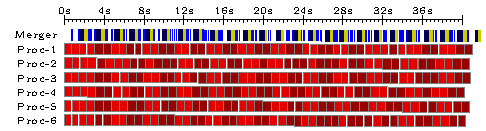
\includegraphics[height=4cm, width=12cm]{plots/old.pdf} \\
		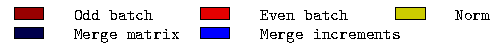
\includegraphics[scale=1]{plots/legend_old.pdf}
	\end{tabular}
	\caption{Gantt chart for execution of the old online algorithm from BigARTM \kw{v0.6}} \label{fig:gantt:oldonline}
\end{figure}

\begin{figure}[h]
	\centering
	\begin{tabular}{c}
		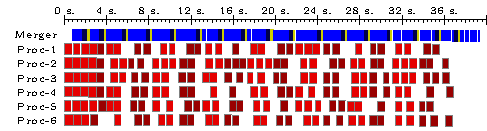
\includegraphics[height=4cm, width=12cm]{plots/old_slow.pdf} \\
		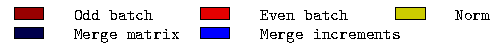
\includegraphics[scale=1]{plots/legend_old.pdf}
	\end{tabular}
	\caption{Gantt chart for execution of the old online algorithm from BigARTM \kw{v0.6}} \label{fig:gantt:oldonlineslow}
\end{figure}

\end{document}


